\documentclass[aps, prb, twocolumn, a4paper, floatfix, reprint]{revtex4-2}
\usepackage[%
    margin=10mm,% ако не си принтира 10мм не изглежда грозно, а може да събереш повече текст
    % showframe=true,%
    ]{geometry}
\usepackage[T1,T2A]{fontenc}
\usepackage[utf8]{inputenc}
\usepackage[main=bulgarian, english]{babel}
\usepackage{float}
\AtBeginDocument{\selectlanguage{bulgarian}}
\newcommand{\degree}{^{\circ}}
\usepackage{amsmath}
\usepackage{graphics}
\usepackage{graphicx}
\graphicspath{{.}}
\newcommand{\abs}[1]{\lvert#1\rvert}
\let\phi\varphi
\usepackage{booktabs} % от тук се използва само \midrule може и без него 
%\usepackage{adjustbox} % това може да се използва, за да „смаляваш“ широки таблици
%\usepackage{tabularx} % дефинира колона X в среда tabularx която добавя празно място така че цялата таблица да запълни определена ширина
\usepackage{dcolumn}
\newcolumntype{d}[1]{D{.}{.}{#1}}
\usepackage[unicode=true,pdfusetitle]{hyperref}


\makeatletter
\renewcommand{\Dated@name}{}%
\makeatother



\begin{document}
\title{Махало на Максуел}
\author{Васил Николов}
\noaffiliation
\date{25.12.2021}
\maketitle

\section{Цел на упражнението}
Да се изследва поведението на махалото на Максуел и да се измери инерчният му момент, както и този на пръстените, които могат да се прикачат към него. 

\section{Експериментална установка}
Махалото на Максуел представлява метален цилиндър, през центъра на който преминава тънка метална ос с фиксиран радиус. На оста от двете страни са намотани тънки неразтегливи нишки. Горните краища на нишките са закрепени на една и съща височина, а между тях има електромагнит и фотоклетка, която засича кога махалото е пуснато, и пуска таймер. В долната част на уреда има втора фотоклетка, която засича преминаването на махалото и спира таймера. Тъи като махалото има значим инерчен момент то пада с ускорение $a$, значително по малко от земното ускорение $g$. $a$ зависи от лесно измерими параметри на системата като радиусът на оста на навиване на нишката $R$ и масата на махалото $m$. Ускорението зависи и от инерчният момент на махалото, и когато измерим времето за падане от фиксирана височина може да се намери ускорението и оттам инерчният момент. 

\section{Теоретична обосновка}
Нека $\vec{r}_i$ е радиусвекторът на точка с пореден номер $i$, а $\Delta t = 1/f$ е времевият интервал между две точки. Тогава средната скорост и средното ускорение на тялото в точка $i$ е 
\begin{subequations} \label{eq:1} 
\begin{gather} 
    \vec{v_i} = \frac{\vec{r}_{i + 1} - \vec{r}_{i - 1}}{2\Delta t} \\
    \vec{a_i} = \frac{\vec{v}_{i + 1} - \vec{v}_{i - 1}}{2\Delta t} 
\end{gather}
\end{subequations}

\section{Обработка на данните}
Листът, на който са точките се снима, и дигитално се снемат коордитатите на точките в пиксели. На листа се нанася и мащаб - отсечка, чиято дължина знаем. Като се снемат краищата на отсечката като още две точки може да се определи мащабът на снимката, и да се пресметне на какви координати в сантиметри отговарят координатите в пиксели. След това по формулите, описани в \eqref{eq:1} се пресмятат векторите на ускорението и скоростта. На снимката се нанасят вектори с начало избраните точки с дължина, пропорционална на съответно скоростта и ускорението. За целта се избира такъв мащаб, че стрелките да не се припокриват много, но и да не са твърде къси. 

\section{Експериментални данни и резултати}

На фигурата с червени стрелки е скоростта на главата, а със сини - ускорението й. Посоките на скоростта и ускорението във всяка точка съвпадат с очакванията ни.
\begin{figure}[h]
    \caption{Скорост и ускорение при криволинейно движение}
    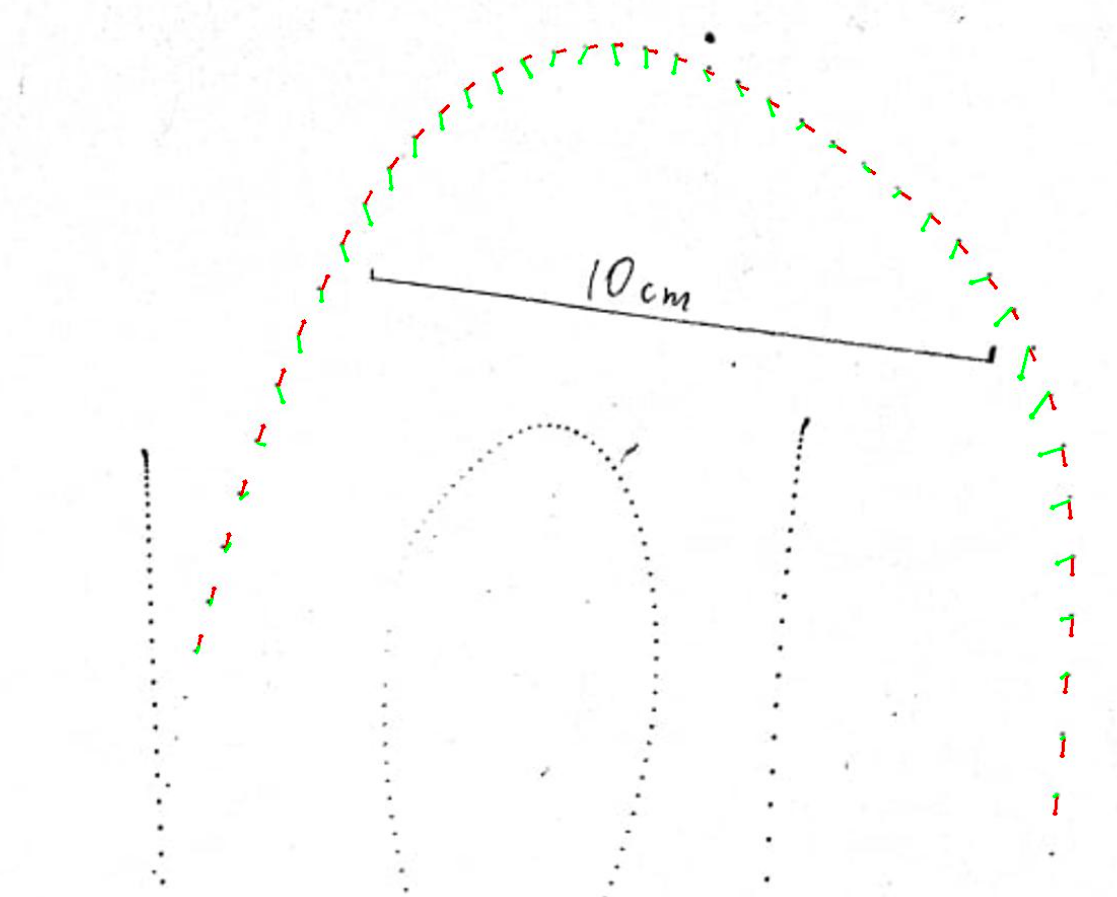
\includegraphics[width=0.9\columnwidth,keepaspectratio=true]{cropped_velocity_acceleration.png}
\end{figure}

\begin{figure}[H]
    \caption{Скорост при праволинейно движение на тялото}
    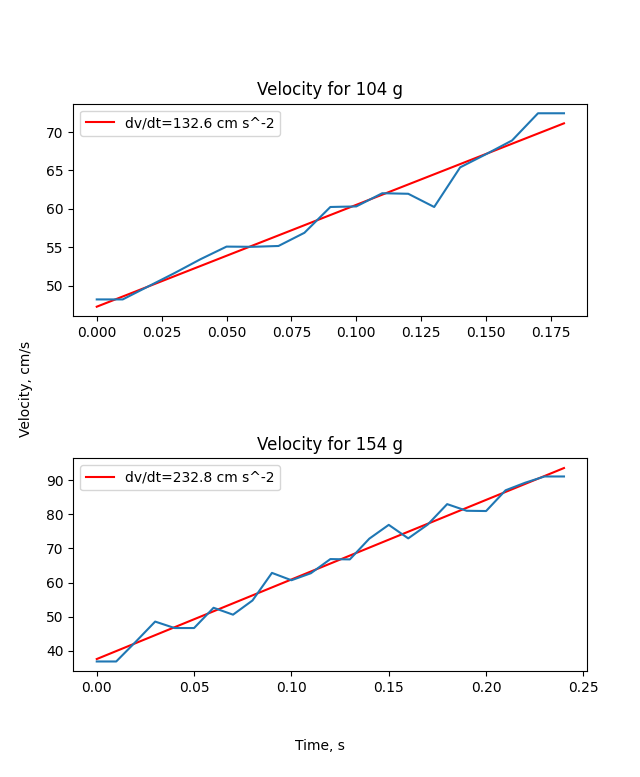
\includegraphics[width=0.9\columnwidth,keepaspectratio=true]{vel_charts_3.png}
\end{figure}

На двете графики са дадени скоростта и ускорението на тялото когато се дърпа от съответно $104 g$ и $154 g$. При снемане на позиции на точките, особено когато разстоянието между тях е малко, се натрупва голяма грешка при измерване, заради която графиката не е идеална права, и пресметнатото ускорение не е близко до очакваното постоянно ускорение. Заради това графика на ускоренията от времето не са представени. 


\end{document}